%SVN info for this file
\svnidlong
{$HeadURL$}
{$LastChangedDate$}
{$LastChangedRevision$}
{$LastChangedBy$}

\chapter{Proprietà magnetiche della materia}
\labelChapter{magnetismoMateria}

\begin{introduction}
	``Water, fire, air and dirt\\
	Fucking magnets, how do they work?\\
	And I don’t wanna talk to a scientist\\
	Y’all motherfuckers lying, and getting me pissed''
	\begin{flushright}
		\textscsl{Insane Clown Posse}, vincitori del premio Nobel per la fisica del 2009.
	\end{flushright}
\end{introduction}
\lettrine[findent=1pt, nindent=0pt]{S}{e chiedete} alla prima persona per strada che cos'è il ``magnetismo'', probabilmente la sua risposta riguarderà bussole, Poli e magneti a ferro di cavallo - hey, proprio come quello in copertina! Insomma, tutto quello che abbiamo raccontato da un punto di vista storico all'inizio del \autoref{chap:campoMagnetico}, ma difficilmente sentirete parlare di cariche in movimento o, sia mai, fili percorsi da corrente.\\
Eppure, tutti i fenomeni magnetici sono dovuti a \textit{cariche elettriche in moto} e, infatti, se esaminassimo su scalato atomica un pezzettino di materiale magnetico troveremmo delle correnti piccole piccole: gli elettroni che orbitano attorno al nucleo\footnote{O meglio, gli elettroni non girano intorno all'atomo esattamente come nela bandiera di Železnogorsk, in Russia, ma si dispongono sui livelli energetici degli orbitali. Se non conoscete quella bandiera cercatela, è spettacolare.} e gli elettroni che roteano attorno ai loro assi. Queste correnti formano, con buona ma forse troppa approssimazione, delle minuscole spire che generano un dipolo magnetico. Normalmente, gli atomi sono orientati casualmente e questi piccoli campi si cancellano a vicenda... ma quando un campo magnetico esterno viene applicato, questi dipoli si allineano e il materiale si \textit{magnetizza}. Però, come tutto in Fisica, non è così facile come sembra.

In questo Capitolo ci dedicheremo a tutto che riguarda la \textbf{magnetizzazione dei materiali}: facendo dei confronti con la polarizzazione dei dielettrici parleremo della \textbf{permeabilità magnetica} e dei \textbf{processi di magnetizzazione}. Riprenderemo poi le \textbf{leggi di Maxwell per l'elettromagnetismo} adattandole al caso dei materiali isolanti e paramagnetici/diamagnetici. In conclusione accenneremo leggermente il complicato ma curioso funzionamento dei \textbf{ferromagneti}.
\section{Permeabilità magnetica e suscettività magnetica}
\begin{comment}
Come si comporta il campo magnetico all'interno dei materiali?\\
Valgono tutti i caveat già visti nell'elettricità nei materiali dielettrici.\\
Per avere un modello realistico serve un modello quantistico, gli altri infatti non hanno un valore quantitativo.\\
Nel caso dielettrico partendo da osservazioni macroscopiche, deduciamo meccanismi sulle proprietà materiali e poi non ci addentreremo nei meccanismi microscopici, per cui serve quantistica. Per quanto riguarda gli aspetti magnetici delle particelle microscopiche dipendono (?)
Un campo magnetico si accoppia ad una particella solo se questa è carica ed è in moto, che prende momento magnetico se, nel caso della spira, si muove di moto circolare.\\
Un'interpretazione che possiamo dare è ch l'elettrone nella sua rotazione intorno al  nucleo, produce un momento angolare che si allinea con il campo magnetico, ma questo è errato dal punto di vista quantitativo,infatti l'elettrone non gira intorno all'atomo ma si dispone sui livelli energetici degli orbitali.\\
Inoltre gli elettroni hanno anche momento angolare intrinseco (analogo alla rotazione su sè stesso), ed è lo \textit{spin} \index{spin}. Esso è una caratteristica intrinseca, che produce un momento di dipolo magnetico che si accoppia con il campo magnetico e si allinea.\\
La descrizione classica dei momenti di dipolo magnetico che si allineano o disallineano dà un'intuizione, ma per una comprensione efficace fenomeni servono modelli statistici e quantistici che non abbiamo e non tratteremo in questo corso.
\end{comment}
\begin{remember}
Prendiamo un \textit{condensatore} che genera tra le armature cariche un campo elettrico costante $E_0$. Se poniamo all'interno una lastra di \textit{materiale dielettrico}, il campo elettrico effettivo misurato tra le piastre diventa
\begin{equation*}
	E_\kappa=\frac{E_0}{\kappa}=\frac{\sigma}{\kappa\epsilon_0}=\frac{\sigma}{\epsilon}
\end{equation*}
dove con $\kappa>1$ è la \textit{costante dielettrica relativa}, dipendente dal materiale, e
\begin{equation*}
	\epsilon=\kappa \epsilon_0
\end{equation*}
la \textit{costante dielettrica assoluta}.
\end{remember}
\noindent Consideriamo un apparato per generare un campo magnetico costante $\vba{B}_0$, come ad esempio un solenoide cilindrico di $n$ spire percorso da una corrente $I$, e lo riempiamo di un certo mezzo omogeneo.
\begin{center}
	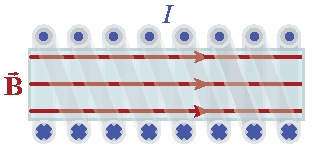
\includegraphics[width=0.75\textwidth]{images/chp12/chp12solenoideriempito1.pdf}
\end{center}
Ul campo $\vba{B}$ che misuriamo ora in presenza del materiale è parallelo e concorde a $\vba{B}_0$; inoltre, il rapporto tra i moduli del campo magnetico nel vuoto e di quello misurato nel mezzo è
\begin{equation*}
	\kappa_m=\frac{B_{\kappa_m}}{B_0}
\end{equation*}
Sperimentalmente, si trova che tale rapporto è \textit{caratteristico} del \textit{tipo} di materiale e non dipende dalla geometria o dalla corrente del solenoide.
\begin{define}[Costante di permeabilità magnetica relativa e suscettibilità elettrica del dielettrico]
	La \textbf{costante di permeabilità magnetica relativa}\index{costante!di permeabilità magnetica!relativa} è il rapporto adimensionale
	\begin{equation}
		\tcboxmath[colback=yellowpastellow!30!white,colframe=ceruleancrayola!85!black,drop fuzzy shadow, nobeforeafter, math upper, tcbox raise base, enhanced]{\kappa_m=\frac{B_{\kappa_m}}{B_0}}\label{CostantePermRelativaDef}
	\end{equation}
	La grandezza
	\begin{equation}
		\tcboxmath[colback=yellowpastellow!30!white,colframe=ceruleancrayola!85!black,drop fuzzy shadow, nobeforeafter, math upper, tcbox raise base, enhanced]{\chi_m=\kappa_m - 1>0}
	\end{equation}
	viene detta \textbf{suscettibilità magnetica}\index{suscettibilità!magnetica}, mentre la grandezza
	\begin{equation}
		\tcboxmath[colback=yellowpastellow!30!white,colframe=ceruleancrayola!85!black,drop fuzzy shadow, nobeforeafter, math upper, tcbox raise base, enhanced]{\mu=\kappa_m\mu_0}
	\end{equation}
	è definita \textbf{permeabilità magnetica assoluta}\index{costante!di permeabilità magnetica!assoluta}
\end{define}
La situazione è all'apparenza analoga a quella dei dielettrici: il rapporto tra campo magnetico misurato nel mezzo e quello nel vuoto dipende solo dal materiale e risulta esserci una relazione lineare tra di essi.
La grossa differenza rispetto al caso elettrico è che $\kappa_m$ \textit{non} è sempre maggiore di $1$! Infatti, possiamo classificare i materiali in base alla loro permeabilità magnetica:
\begin{itemize}
	\item Se $\kappa_m<1\ (\chi_m<0)$ il materiale è detto \textbf{diamagnetico}\index{diamagnetismo}\index{materiale!diamagnetico}: il campo magnetico nel mezzo è meno intenso di quello nel vuoto.
	\begin{equation}
		\tcboxmath[colback=yellowpastellow!30!white,drop fuzzy shadow, nobeforeafter, math upper, tcbox raise base, enhanced]{B_{\kappa}<B_0}
	\end{equation}
	\item Se $\kappa_m>1\ (\chi_m>0)$ il materiale è detto \textbf{paramagnetico}\index{paramagnetismo}\index{materiale!paramagnetico}: il campo magnetico nel mezzo è meno intenso di quello nel vuoto.
	\begin{equation}
		\tcboxmath[colback=yellowpastellow!30!white,drop fuzzy shadow, nobeforeafter, math upper, tcbox raise base, enhanced]{B_{\kappa}>B_0}
	\end{equation}
	\item Se $\kappa_m\gg 1$ (circa nell'ordine di $10^5$) il materiale è detto \textit{ferromagnetico}\index{ferromagnetismo}\index{materiale!ferromagnetico}. Questo caso esula da quelli precedenti: $\kappa_m$ non è più un valore \textit{costante} (anzi, varia sensibilmente valore!), ma dipende da \textit{come viene magnetizzato}\footnote{Nella sezione \ref{ferromagnetici}, pag. \pageref{ferromagnetici} approfondiremo i materiali ferromagnetici e come si magnetizzano.} il materiale.
\end{itemize}
\begin{examplewt}[Valori della suscettibilità magnetica]
	\begin{center}
		\begin{tabular}{l|c|l|c}
			\textbf{Diamagneti} & $\chi_m$ & \textbf{Paramagneti} & $\chi_m$\\
			\hline
			Argento & \num{2,39d-5} 	& Alluminio & \num{2,08d-5}\\
			Oro 	& \num{-3,46d-5} 	& Platino 	& \num{2,791d-5}\\
			Rame 	& \num{-0,98d-5} 	& Uranio 	& \num{40,92d-5}
		\end{tabular}
	\end{center}
\end{examplewt}
\section{Magnetizzazione}
\begin{remember}
	Il campo elettrostatico nei materiali dielettrici è dovuto a fenomeni di \textit{polarizzazione}, in cui le particelle del materiale acquistano un momento di dipolo proporzionale ad un campo elettrico esterno in modo da verificare i fenomeni osservati. Ci eravamo concentrati su due tipi di polarizzazioni:
	\begin{itemize}
		\item \textbf{Polarizzazione elettronica.} Il campo elettrico esterno causa una \textit{separazione atomica} in cui il centro di carica della nube di elettroni e del nucleo \textit{non} coincidono più, producendo un microscopico momento di dipolo \textit{concorde} al campo elettrico. Gli effetti complessivi dei dipoli causano un \textit{campo elettrico di polarizzazione} parallelo ma \textit{opposto} al campo elettrico esterno.
		\item \textbf{Polarizzazione per orientamento.} In un materiale le cui particelle sono già dotate di un \textit{momento di dipolo nativo} - di norma con orientazione \textit{puramente casuale} a causa dell'agitazione termica - il campo elettrico esterno causa l'allineamento di queste con esso. Come prima, gli effetti complessivi dei dipoli causano un \textit{campo elettrico di polarizzazione} parallelo ma \textit{opposto} al campo elettrico esterno.
	\end{itemize}
In entrambi i casi, il momento di dipolo complessivo è concorde con il campo esterno, mentre il campo elettrico di polarizzazione ad esso associato risulta essere \textit{opposto} al campo esterno
\end{remember}
Il processo che nei materiali para/diamagnetici causa il campo magnetico all'interno del mezzo prende il nome di \textbf{magnetizzazione}\index{magnetizzazione}: esso consiste nel far acquisire alle particelle del materiale un \textit{momento (di dipolo) magnetico} in modo da ottenere il comportamento osservato in precedenza. Ci sono diversi metodi di magnetizzazione, ma i più importanti sono la \textit{magnetizzazione atomica} e la \textit{magnetizzazione per orientamento}.\\
Nell'introduzione abbiamo accennato il punto di collegamento tra quanto visto con i fili percorsi da corrente e il mondo microscopico. Ciò nonostante, quella interpretazione è un poco euristica: la trattazione di questi fenomeni è particolarmente complessa e non possiamo addurre loro una spiegazione \textit{quantitativa e precisa} nel \textit{modello classico} - sarà possibile farlo correttamente nell'ambito della Fisica Quantistica. Saremo quindi sintetici sul loro funzionamento.
\begin{itemize}
	\item \textbf{Magnetizzazione atomica.} Il moto degli elettroni attorno al nucleo può essere assimilato a correnti microscopiche, a cui è associato un momento magnetico. Sebbene normalmente questi momenti si compensino, in presenza di un campo magnetico esterno il moto degli elettroni è perturbato e si produce un microscopico momento magnetico non nullo. Nel materiale, gli effetti complessivi di questi momenti causano un \textit{campo magnetico} parallelo ma opposto al campo magnetico esterno. La magnetizzazione atomica ha un effetto \textit{smagnetizzante} ed è la causa dei fenomeni \textit{diamagnetici}.\\
	\begin{minipage}{0.49\textwidth}
		\begin{center}
			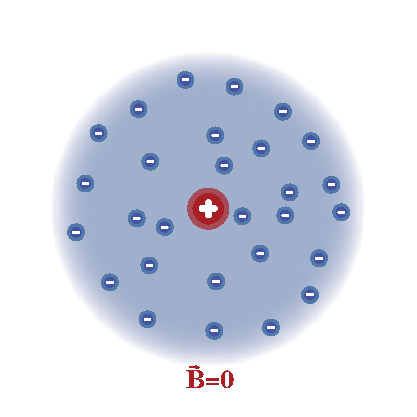
\includegraphics[width=0.75\textwidth]{images/chp12/chp12polarizzazionenucleo1.pdf}
		\end{center}
	\end{minipage}
	\begin{minipage}{0.49\textwidth}
		\begin{center}
			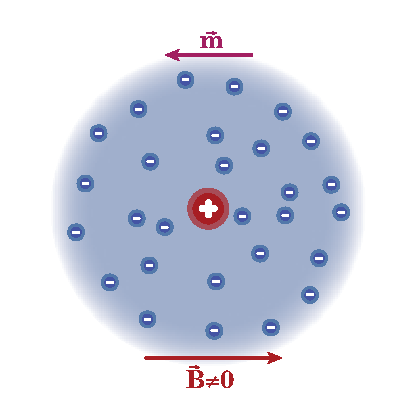
\includegraphics[width=0.75\textwidth]{images/chp12/chp12polarizzazionenucleo2.pdf}
		\end{center}
	\end{minipage}
	\item \textbf{Magnetizzazione per orientamento.} In un materiale le cui particelle sono già dotate di \textit{momenti magnetici nativi} $\vba{m}_i$ - di norma con orientazione \textit{puramente casuale} a causa dell'agitazione termica - il campo magnetico esterno causa l'allineamento di queste con esso. Gli effetti complessivi dei momenti causano un \textit{campo magnetico} parallelo e \textit{concorde} al campo di magnetico esterno. La magnetizzazione per orientamento è la causa dei fenomeni \textit{paramagnetici}.\\
	\begin{minipage}{0.49\textwidth}
		\begin{center}
			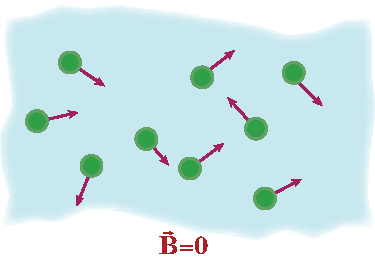
\includegraphics[width=0.75\textwidth]{images/chp12/chp12orientamento1.pdf}
		\end{center}
	\end{minipage}
	\begin{minipage}{0.49\textwidth}
		\begin{center}
			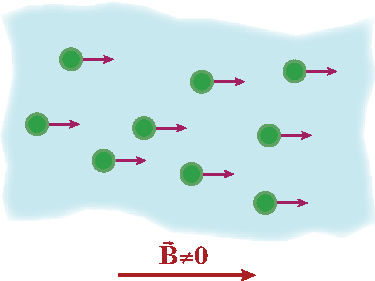
\includegraphics[width=0.75\textwidth]{images/chp12/chp12orientamento2.pdf}
		\end{center}
	\end{minipage}
\end{itemize}
Ecco ``spiegato'' \textit{qualitativamente} il perché del valore così vario di $\kappa_m$: a seconda di quale effetto dei due \textit{prevale} in un dato materiale, esso sarò diamagnetico o parametrico.
\paragraph{Magnetizzazione dei materiali}
In qualunque caso di magnetizzazione ci troviamo, gli atomi o le molecole in un volumetto $\Delta V$ del materiale acquistano, sotto l'azione del campo magnetico esterno $\vba{B}$, un \textit{momento magnetico medio} $\left<\vba{m}\right>$ orientato parallelamente a $\vba{B}$:
\begin{equation}
	\tcboxmath[colback=yellowpastellow!30!white,drop fuzzy shadow, nobeforeafter, math upper, tcbox raise base, enhanced]{\left<\vba{m}\right>=\frac{1}{N}\sum_{i=1}^{N}\vba{m}_i}
\end{equation}
Qui $N$ è il numero di particelle nel volume $\Delta V$. La \textbf{densità di magnetizzazione}\index{densità!di magnetizzazione} risulta
\begin{equation}
	\tcboxmath[colback=yellowpastellow!30!white,drop fuzzy shadow, nobeforeafter, math upper, tcbox raise base, enhanced]{\vba{M}=\frac{\sum_{i=1}^{N}\vba{m}_i}{dV}=\frac{dN\left<\vba{m}\right>}{dV}=n\left<\vba{m}\right>}
\end{equation}
dove
\begin{equation*}
	n=\frac{N}{\Delta V}
\end{equation*}
è la densità di particelle nell'intorno di $Q$.\\
Normalmente, in assenza di campo magnetico la causalità dei momenti fa si che
\begin{equation*}
	\left<\vba{m}\right>=0\implies \vba{M}=0
\end{equation*}
ma se siamo in presenza di un campo magnetico esterno $\vba{B}$ il momento magnetico per unità di volume \textit{non} è nullo ed è allineato con $\vba{B}$:
\begin{equation*}
	\left<\vba{m}\right>\neq 0\implies \vba{M}\neq 0
\end{equation*}
\subsection{Campo magnetico generato dalla magnetizzazione}
\begin{remember}
	Nei materiali \textit{dielettrici} attraversati da un \textit{campo elettrico esterno} - generato da un condensatore - si poteva addurre il \textit{campo di polarizzazione opposto} a delle cariche ``fittizie'' (che poi così fittizie non sono) depositate nel dielettrico con segno opposto a quello della carica libera sul conduttore.
\end{remember}
\noindent Dalla \eqref{CostantePermRelativaDef} scriviamo
\begin{equation*}
	B=\kappa_m B_0=\left(1+\chi_m\right)B_0=B_0+\chi_mB_0=\mu_0 n I + \mu_0 \chi_m n I
\end{equation*}
Dato che il termine $\mu_0 n I$ è il campo magnetico prodotto nel solenoide dalla corrente $I$ che circola nelle spire, il secondo termine rappresenta l'effetto sul campo magnetico misurato da parte del \textit{mezzo magnetizzato} - effetto identico a quello prodotto da un secondo solenoide uguale al primo, ma percorso da una corrente ``fittizie'', detta \textbf{corrente amperiana}\index{corrente elettrica!amperiana}, di intensità
\begin{equation}
	\tcboxmath[colback=yellowpastellow!30!white,drop fuzzy shadow, nobeforeafter, math upper, tcbox raise base, enhanced]{I_m=\chi_m I}
\end{equation}
Se la corrente amperiana è \textit{discorde} rispetto a quella del solenoide il campo misurato è minore di quello nel vuoto e si è in presenza di  fenomeni \textit{diamagnetici}; viceversa, se la corrente amperiana è concorde allora gli effetti si somma e si è verificano fenomeni \textit{paramagnetici}.\\
\begin{minipage}{0.49\textwidth}
	\begin{center}
		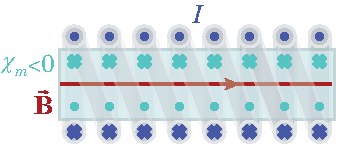
\includegraphics[width=1\textwidth]{images/chp12/chp12solenoideriempito2a.pdf}
	\end{center}
\end{minipage}
\begin{minipage}{0.49\textwidth}
	\begin{center}
		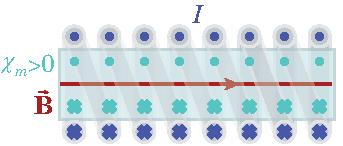
\includegraphics[width=1\textwidth]{images/chp12/chp12solenoideriempito2b.pdf}
	\end{center}
\end{minipage}\\
Vedremo che questa corrente non è ``fittizia'': anche se non è una corrente di conduzione, essa è il risultato macroscopico di \textit{correnti di origini atomiche}.
\paragraph{Modellizzazione delle correnti amperiane - il caso uniforme}
Consideriamo la situazione del solenoide ``pieno''. Il cilindro interno di materiale \textit{magnetizzato uniformemente} ha una densità magnetica $\vba{M}=\text{const}$ parallela all'asse $z$. Supponiamo di suddividerlo in dischi di altezza $dz$ e, a loro volta, li suddividiamo in prismi infinitesimi di base $d\Sigma$, altezza $dz$ e volume $dV=d\Sigma dh$. Ciascuno dei prismi ha un momento magnetico orientato come $\vba{M}$ e pari a
\begin{equation*}
	d\vba{m}=\vba{M}dV=\abs{\vba{M}}d\Sigma d\vba{h}=\abs{\vba{M}} d\Sigma dz\vba{u}_z\label{corrAmp1}
\end{equation*}
Per il \textit{principio di equivalenza di Ampère}\footnote{Si veda \autoref{chap:campoMagnetico}, sezione \ref{principio di equivalenza di ampere}, pag. \pageref{principio di equivalenza di ampere}.} al prisma magnetizzato possiamo sostituire una spira infinitesima di area $d\Sigma$ e altezza $dh$, attraversata da una corrente $dI_m$, il cui momento di dipolo magnetico è pari a $d\vba{m}$ ed è tale per cui
\begin{equation*}
	d\vba{m}=dI_md\Sigma \vbh{u}_z \label{corrAmp2}
\end{equation*}
\begin{center}
	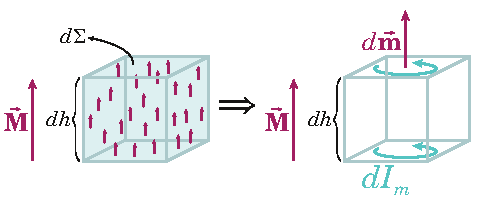
\includegraphics[width=0.75\textwidth]{images/chp12/chp12momento1.pdf}
\end{center}
Uguagliando la \eqref{corrAmp1} e la \eqref{corrAmp2} otteniamo
\begin{equation}
	\tcboxmath[colback=yellowpastellow!30!white,drop fuzzy shadow, nobeforeafter, math upper, tcbox raise base, enhanced]{dI_m=\abs{\vba{M}}dz}\label{correnteampdisc}
\end{equation}
Siccome supponiamo $\vba{M}$ uniforme su tutto il dielettrico, il vettore di magnetizzazione è lo stesso per due prismi \textit{contigui}, di conseguenza l'intensità della corrente amperiana infinitesima è costante in tutta l'oggetto. Sulle \textit{superfici di contatto} tra prismi tali corrente sono \textit{uguali e contrarie}, quindi si elidono a due a due. Le uniche correnti non bilanciate sono quelle sulla \textit{superficie esterna} del disco: il disco di materiale magnetizzato uniformemente è equivalente ad un circuito percorso dalla corrente \eqref{correnteampdisc}.
\begin{center}
	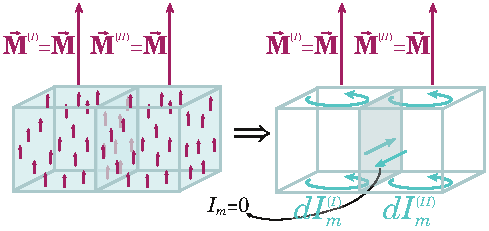
\includegraphics[width=0.75\textwidth]{images/chp12/chp12momento2.pdf}
\end{center}
Ripetendo il ragionamento con i dischi, il cilindro è equivalente ad un circuito di altezza $h$ percorso dalla corrente amperiana
\begin{equation}
		\tcboxmath[colback=yellowpastellow!30!white,drop fuzzy shadow, nobeforeafter, math upper, tcbox raise base, enhanced]{I_m=\int_{0}^{h}\abs{\vba{M}}dz=\abs{\vba{M}}h}
\end{equation}
\begin{center}
	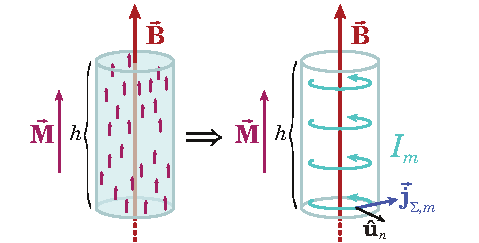
\includegraphics[width=0.75\textwidth]{images/chp12/chp12momento3.pdf}
\end{center}
\begin{remember}
	La densità superficiale delle cariche di polarizzazione è
	\begin{equation}
		\sigma_p=\vba{P}\vdot\vbh{u}_n
	\end{equation}
\end{remember}
\noindent La situazione magnetica è \textit{duale} a quella del dielettrico. Infatti, possiamo definire una grandezza vettoriale associata alla corrente amperiana detta \textbf{densità lineare di corrente}\index{densità!di corrente!superficiale}:
\begin{equation}
	\tcboxmath[colback=yellowpastellow!30!white,drop fuzzy shadow, nobeforeafter, math upper, tcbox raise base, enhanced]{\vba{j}_{\Sigma, m}=\vba{M}\cross\vbh{u}_n}\label{CorrenteAmpereUnif}
\end{equation}
il cui verso è regolato dalla regola della mano destra.
\begin{attention}
	La densità di corrente amperiana nel caso uniforme, sebbene circoli soltanto sulla superficie, è di natura \textit{lineare}! Infatti, la corrente amperiana circola soltanto su \textit{anelli lineari} (tutti paralleli tra di loro) del cilindro e quindi anche la densità è lineare per questo motivo.
\end{attention}
\paragraph{Modellizzazione delle correnti amperiane - il caso \textit{non} uniforme}
\begin{remember}
	Se il vettore di polarizzazione \textit{non} è uniforme, le cariche di polarizzazione sono presenti anche all'\textit{interno} del dielettrico.
\end{remember}
\noindent Se il vettore di magnetizzazione \textit{non} è uniforme, la carica amperiana \textit{non} scorre solo sulla superficie. Consideriamo sempre la suddivisione in prismi infinitesimi in modo che in ogni prisma il vettore di magnetizzazione ha un valore costante. Vogliamo studiare il valore della corrente amperiana lungo la direzione $y$; essendo $\vba{M}$ non uniforme, i contributi alla corrente amperiana provengono da molteplici direzioni.\\
Prendiamo la \textit{base comune} a due prismi contigui lungo l'asse $x$ e con area di base $d\Sigma=dxdz$. In ciascun prisma, alla componente $M_z(x)$ di $\vba{M}$ è associata una corrente $I_y^{(1)}$ opportuna secondo l'\textit{equivalenza di Ampere}. La corrente complessiva sulla superficie di contatto dati questi due elementi è
\begin{equation*}
	I_y^{(1)}=I_1^{(I)}-I_2^{(II)}=\left(M_z(x)-M_z(x+dx)\right)dz=\left(M_z^{(I)}-M_z^{(II)}\right)dz=-\pdv{M_z}{x}dxdz
\end{equation*}
\begin{center}
	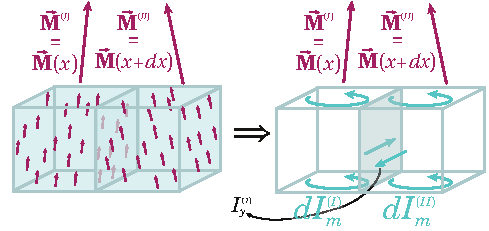
\includegraphics[width=0.75\textwidth]{images/chp12/chp12momento4.pdf}
\end{center}
In realtà non è l'unico contributo lungo l'asse $y$. Infatti, consideriamo un'altra coppia di prismi, questa volta contigui lungo l'asse $z$ e con area di base $d\Sigma=dxdz$. In ciascun prisma, la componente $M_x(z)$ di $\vba{M}$ è prodotta da un'opportuna corrente amperiana $I_y^{(2)}$ lungo $y$:
\begin{equation*}
	I_y^{(2)}=I_1^{(I)}-I_2^{(II)}=\left(M_x(z)-M_x(z+dz)\right)dz=\left(M_z^{(I)}-M_z^{(II)}\right)dz=-\pdv{M_x}{z}dxdz
\end{equation*}
\begin{center}
	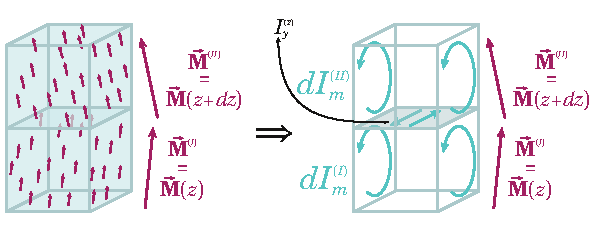
\includegraphics[width=0.75\textwidth]{images/chp12/chp12momento5.pdf}
\end{center}
Si osserva invece che la componente $M_y(y)$ è \textit{uniforme} in entrambi i casi affrontati e, d'altro canto, non ha rilevanza per le correnti amperiane perché tale situazione è riconducibile a quella già vista in cui le correnti interne si semplificano.\\
In totale, lungo l'asse $y$ la corrente è
\begin{equation}
	I_y=I_y^{(1)}+I_y^{(2)}=\left(\pdv{M_x}{z}-\pdv{M_z}{x}\right)dxdz=\left(\curl{\vba{M}}\right)_ydxdz
\end{equation}
Si nota inoltre che l'elemento di area è ortogonale all'asse $y$, quindi la componente lungo $y$ della densità di corrente è
\begin{equation*}
	j_y=\frac{dI_y}{dxdz}\left(\pdv{M_x}{z}-\pdv{M_z}{x}\right)=\left(\curl{\vba{M}}\right)_y
\end{equation*}
Riapplicando il ragionamento anche nelle altre direzioni otteniamo
\begin{equation}
		\tcboxmath[colback=yellowpastellow!30!white,drop fuzzy shadow, nobeforeafter, math upper, tcbox raise base, enhanced]{\vba{j}_m=\curl{\vba{M}}}\label{CorrenteAmpereNonUnif}
\end{equation}
Dalle leggi \eqref{CorrenteAmpereUnif} e \eqref{CorrenteAmpereNonUnif} si deduce che gli effetti magnetici di un mezzo magnetizzato si possono calcolare a partire da una distribuzione \textit{superficiale} di corrente con densità \textit{lineare} $\vba{j}_{\Sigma, m}$ e di una distribuzione \textit{spaziale} di corrente con densità $\vba{j}_m$.
\section{Le equazioni di Maxwell nei materiali}
Siamo ora in grado di formulare le equazioni della magnetostatica nei materiali: dovremo modificare quelle leggi che presentano al loro interno informazioni riguardo le sorgenti di campo.\\
Consideriamo un campo magnetostatico $\vba{B}$. Mentre la divergenza del campo magnetico rimane nulla...
\begin{equation}
	\div{\vba{B}}=0
\end{equation}
... il suo rotore risulta pari alla densità di corrente complessiva $\vba{j}_{tot}$ nel materiale, moltiplicata per $\mu_0$ - ma tale densità è pari alla somma di quella di conduzione $\vba{j}$ già presente e di quella corrente amperiana $\vba{j}_m$:
\begin{equation*}
	\curl{\vba{B}}=\mu_0\vba{j}_{tot}=\mu_0\left(\vba{j}+\vba{j}_m\right)=\mu_0\vba{j}+\mu_0\curl{\vba{M}}=\implies \curl{\left(\frac{\vba{B}}{\mu_0}-\vba{M}\right)}=\vba{j}
\end{equation*}
Definito il \textbf{campo magnetizzante}\index{campo!magnetizzante}
\begin{equation}
		\tcboxmath[colback=yellowpastellow!30!white,drop fuzzy shadow, nobeforeafter, math upper, tcbox raise base, enhanced]{\vba{H}=\frac{\vba{B}}{\mu_0}-\vba{M}}
\end{equation}
otteniamo la legge
\begin{equation}
		\tcboxmath[colback=yellowpastellow!30!white,drop fuzzy shadow, nobeforeafter, math upper, tcbox raise base, enhanced]{\curl{\vba{H}}=\vba{j}}\label{QuartaMaxwellMagnetUno}
\end{equation}
\begin{observe}
	Quando consideriamo un materiale diamagnetico o paramagnetico immerso in un campo magnetico $\vba{B}$, ciò che andiamo a modificare è il campo magnetizzante $\vba{H}$ e non $\vba{B}$.
\end{observe}
\begin{attention}
	Il campo magnetizzante $\vba{H}$ è soltanto un campo ausiliario: non ha un vero e proprio significato fisico.
\end{attention}
Ci sembrerebbe di aver fatto ``sparire'' le correnti amperiane riscrivendo la \textit{legge di Ampère per la circuitazione} in questa maniera, ma in realtà l'abbiamo soltanto nascosta sotto il tappeto!\footnote{Come già detto, non invidio chi dovrà lavare tale tappeto.}  I campi $\vba{B}$ e $\vba{H}$ sono legati ancora dalla densità di magnetizzazione $\vba{M}$ - che incorpora in essa le informazioni della corrente amperiana. Per poter risolvere \textit{definitivamente} $\vba{B}$ e $\vba{H}$ ci un'\textbf{equazione di stato del mezzo magnetico}\index{equazione!di stato!del mezzo magnetico} che leghi esplicitamente $\vba{B}$ e $\vba{M}$ o, equivalentemente, $\vba{H}$ e $\vba{B}$. Per molti materiali diamagnetici e paramagnetici vale la seguente relazione \textit{lineare}:
\begin{equation}
		\tcboxmath[colback=yellowpastellow!30!white,drop fuzzy shadow, nobeforeafter, math upper, tcbox raise base, enhanced]{\vba{M}=\chi_m\vba{H}}
\end{equation}
\begin{attention}
	Tale legge non è valida per i \textit{materiali ferromagnetici}.
\end{attention}
\begin{digression}
	Per molti materiali paramagnetici la magnetizzazione $\vba{B}$ è dunque proporzionale al campo magnetizzante $\vba{H}$ se le temperature sono \textit{sufficientemente alte} e i campi \textit{sufficientemente piccoli}. A valori dei campi fissi, la suscettibilità magnetica è inversamente proporzionale alla temperatura secondo la \textbf{prima legge di Curie}\index{legge!di Curie, prima}:
	\begin{equation*}
		\tcboxmath[colback=yellowpastellow!30!white,colframe=ceruleancrayola!85!black,drop fuzzy shadow, nobeforeafter, math upper, tcbox raise base, enhanced]{\chi_m=\frac{C}{T}\sim\frac{\rho}{T}}
	\end{equation*}
	Qui $C$ è una costante detta \textbf{costante di Curie}\index{costante!di Curie} specifica del materiale; per una formula esplicita di tale costante sono richieste conoscenze troppo approfondite di Fisica Quantistica, ma ci basta sapere che è proporzionale alla densità del materiale $\rho$ (o, più precisamente, al numero di atomi/molecole magnetizzate per unità di volume).
\end{digression}
\noindent Da essa ricaviamo
\begin{equation*}
	\vba{B}=\mu_0\left(\vba{M}+\vba{H}\right)=\mu_0\left(\chi_m+1\right)\vba{H}=\mu_0\kappa_m\vba{H}=\mu\vba{H}
\end{equation*}
\begin{equation}
		\tcboxmath[colback=yellowpastellow!30!white,drop fuzzy shadow, nobeforeafter, math upper, tcbox raise base, enhanced]{\vba{B}=\kappa_m\mu_0\vba{H}=\mu\vba{H}}
\end{equation}
e la \eqref{QuartaMaxwellMagnetUno} si può riscrivere come
\begin{equation}
	\tcboxmath[colback=yellowpastellow!30!white,drop fuzzy shadow, nobeforeafter, math upper, tcbox raise base, enhanced]{\curl{\vba{B}}=\mu\vba{j}}
\end{equation}
\begin{observe}
	L'ultima legge è pari all'analoga equazione della magnetostatica nel vuoto a cui abbiamo sostituito a $\mu_0$ la costante assoluta $\mu$.
\end{observe}
\paragraph{Leggi di Maxwell per l'elettromagnetostatica nei materiali}
Ricapitolando, si hanno le seguenti leggi nel caso di un materiale qualunque...
\begin{center}
	\begin{tabular}{p{0.22\textwidth}|c|c}
		\centering{\textbf{Nome}} &
		\textbf{Forma integrale} &
		\begin{tabular}{@{}c@{}} \textbf{Forma} \\ \textbf{differenziale}\end{tabular} \\ \hline
		
		\begin{tabular}[c]{@{}p{0.22\textwidth}@{}}	
			\\[-2mm]\textbf{Legge di Gauss per l'elettricità}\\[-2mm]~
		\end{tabular}
		&
		\begin{tabular}[c]{@{}c@{}}
			\\[-2mm]
			$\displaystyle\Phi_{\partial V}(\vba{D})=\int_{\partial V}\vba{D}\vdot\vbh{u}_nd\Sigma=q_{int}=\int_{V}\rho dV$\\[-2mm]~
		\end{tabular} &
		\begin{tabular}[c]{@{}c@{}}
			\\[-2mm]
			$\displaystyle\div{\vba{D}}=\rho$\\[-2mm]~
		\end{tabular} \\ \hline
		\begin{tabular}[c]{@{}p{0.18\textwidth}@{}}	
		\\[-2mm] \textbf{Legge di Gauss per il magnetismo}\\[-2mm]~
		\end{tabular} &
		\begin{tabular}[c]{@{}c@{}}
		\\[-2mm]
		$\displaystyle\Phi_{\partial V}(\vba{B})=\int_{\partial V}\vba{B}\vdot\vbh{u}_nd\Sigma=0$\\[-2mm]~
		\end{tabular} &
		\begin{tabular}[c]{@{}c@{}}
		\\[-2mm]
		$\displaystyle\div{\vba{B}}=0$\\[-2mm]~
		\end{tabular} \\ \hline
		\begin{tabular}[c]{@{}p{0.22\textwidth}@{}}	
			\\[-2mm] \textbf{Legge dell'induzione di Faraday}\\[-2mm]~
		\end{tabular} &
		\begin{tabular}[l]{@{}l@{}}
			\\[-3mm]
			$\displaystyle\Gamma_{\gamma}(\vba{E})=\oint_{\partial \Sigma} \vba{E}\vdot d\vba{s}=0$\\[-1mm]~
		\end{tabular}
		&
		\begin{tabular}[c]{@{}c@{}}
			\\[-3mm]
			$\displaystyle\curl{\vba{E}}=0$
		\end{tabular} \\ \hline
		\begin{tabular}[c]{@{}p{0.18\textwidth}@{}}	
		\\[-2mm] \textbf{Legge della circuitazione di Ampère-Maxwell}
		\end{tabular} &
		\begin{tabular}[l]{@{}l@{}}
			\\[-3mm]
			$\displaystyle\Gamma_{\gamma}(\vba{H})=\oint_{\partial \Sigma} \vba{H}\vdot d\vba{s}=\int_{\Sigma}\vba{j}\vdot\vbh{u}_nd\Sigma=I_{int}$
		\end{tabular} &
		\begin{tabular}[l]{@{}l@{}}
			\\[-2mm]
			$\displaystyle\curl{\vba{H}}=\vba{j}$
		\end{tabular}
	\end{tabular}
\begin{equation*}
	\textit{dove}\qquad\qquad\epsilon_0\vba{E}=\vba{D}-\vba{P}\qquad\frac{\vba{B}}{\mu_0}=\vba{H}+\vba{M}
\end{equation*}
\end{center}
... e le seguenti per un materiale al contempo dielettrico e diamagnetico/paramagnetico lineare (con \textit{costante dielettrica assoluta} $\epsilon=\kappa\epsilon_0$) e \textit{costante di permeabilità magnetica assoluta} $\mu=\kappa\mu_0$).
\begin{center}
	\begin{tabular}{p{0.22\textwidth}|c|c}
		\centering{\textbf{Nome}} &
		\textbf{Forma integrale} &
		\begin{tabular}{@{}c@{}} \textbf{Forma} \\ \textbf{differenziale}\end{tabular} \\ \hline
		
		\begin{tabular}[c]{@{}p{0.22\textwidth}@{}}	
			\\[-2mm]\textbf{Legge di Gauss per l'elettricità}\\[-2mm]~
		\end{tabular}
		&
		\begin{tabular}[c]{@{}c@{}}
			\\[-2mm]
			$\displaystyle\Phi_{\partial V}(\vba{E})=\int_{\partial V}\vba{E}\vdot\vbh{u}_nd\Sigma=\frac{q_{int}}{\epsilon_0}=\int_{V}\rho dV$\\[-2mm]~
		\end{tabular} &
		\begin{tabular}[c]{@{}c@{}}
			\\[-2mm]
			$\displaystyle\div{\vba{E}}=\frac{\rho}{\epsilon}$\\[-2mm]~
		\end{tabular}  \\ \hline
		\begin{tabular}[c]{@{}p{0.18\textwidth}@{}}	
		\\[-2mm] \textbf{Legge di Gauss per il magnetismo}\\[-2mm]~
		\end{tabular} &
		\begin{tabular}[c]{@{}c@{}}
			\\[-2mm]
			$\displaystyle\Phi_{\partial V}(\vba{B})=\int_{\partial V}\vba{B}\vdot\vbh{u}_nd\Sigma=0$\\[-2mm]~
		\end{tabular} &
		\begin{tabular}[c]{@{}c@{}}
			\\[-2mm]
			$\displaystyle\div{\vba{B}}=0$\\[-2mm]~
		\end{tabular} \\ \hline
		\begin{tabular}[c]{@{}p{0.22\textwidth}@{}}	
			\\[-2mm] \textbf{Legge dell'induzione di Faraday}\\[-2mm]~
		\end{tabular} &
		\begin{tabular}[l]{@{}l@{}}
			\\[-3mm]
			$\displaystyle\Gamma_{\gamma}(\vba{E})=\oint_{\partial \Sigma} \vba{E}\vdot d\vba{s}=0$\\[-1mm]~
		\end{tabular}
		&
		\begin{tabular}[c]{@{}c@{}}
			\\[-3mm]
			$\displaystyle\curl{\vba{E}}=0$
		\end{tabular}  \\ \hline
		\begin{tabular}[c]{@{}p{0.18\textwidth}@{}}	
		\\[-2mm] \textbf{Legge della circuitazione di Ampère-Maxwell}
		\end{tabular} &
		\begin{tabular}[l]{@{}l@{}}
			\\[-3mm]
			$\displaystyle\Gamma_{\gamma}(\vba{B})=\oint_{\partial \Sigma} \vba{B}\vdot d\vba{s}=\mu\int_{\Sigma}\vba{j}\vdot\vbh{u}_nd\Sigma=\mu I_{int}$
		\end{tabular} &
		\begin{tabular}[l]{@{}l@{}}
		\\[-2mm]
			$\displaystyle\curl{\vba{B}}=\mu\vba{j}$
		\end{tabular}
	\end{tabular}
\end{center}
\paragraph{Leggi di Maxwell per l'elettromagnetismo nei materiali}
Non è difficile ricavare le equazioni di Maxwell anche per campi \textit{dipendenti dal tempo}. Si hanno le seguenti leggi nel caso di un materiale qualunque...
\begin{center}
	\begin{tabular}{p{0.18\textwidth}|c|c}
		\centering{\textbf{Nome}} &
		\textbf{Forma integrale} &
		\begin{tabular}{@{}c@{}} \textbf{Forma} \\ \textbf{differenziale}\end{tabular} \\ \hline
		\begin{tabular}[c]{@{}p{0.18\textwidth}@{}}	
			\\[-2mm]\textbf{Legge di Gauss per l'elettricità}\\[-2mm]~
		\end{tabular}
		&
		\begin{tabular}[c]{@{}c@{}}
			\\[-2mm]
			$\displaystyle\Phi_{\partial V}(\vba{D})=\int_{\partial V}\vba{D}\vdot\vbh{u}_nd\Sigma=q_{int}=\int_{V}\rho dV$\\[-2mm]~
		\end{tabular} &
		\begin{tabular}[c]{@{}c@{}}
			\\[-2mm]
			$\displaystyle\div{\vba{D}}=\rho$\\[-2mm]~
		\end{tabular} \\ \hline
		\begin{tabular}[c]{@{}p{0.18\textwidth}@{}}	
			\\[-2mm] \textbf{Legge di Gauss per il magnetismo}\\[-2mm]~
		\end{tabular} &
		\begin{tabular}[c]{@{}c@{}}
			\\[-2mm]
			$\displaystyle\Phi_{\partial V}(\vba{B})=\int_{\partial V}\vba{B}\vdot\vbh{u}_nd\Sigma=0$\\[-2mm]~
		\end{tabular} &
		\begin{tabular}[c]{@{}c@{}}
			\\[-2mm]
			$\displaystyle\div{\vba{B}}=0$\\[-2mm]~
		\end{tabular} \\ \hline
		\begin{tabular}[c]{@{}p{0.18\textwidth}@{}}	
			\\[-2mm] \textbf{Legge dell'induzione di Faraday}\\[-2mm]~
		\end{tabular} &
		\begin{tabular}[l]{@{}l@{}}
			\\[-3mm]
			$\displaystyle\Gamma_{\gamma}(\vba{E})=\oint_{\partial \Sigma} \vba{E}\vdot d\vba{s}=$\\
			$\displaystyle\quad=-\dv{t} \int_{\Sigma}\vba{B}\vdot\vbh{u}_nd\Sigma=-\int_{\Sigma}\pdv{\vba{B}}{t}\vdot\vbh{u}_nd\Sigma$\\[-1mm]~
		\end{tabular}
		&
		\begin{tabular}[c]{@{}c@{}}
			\\[-3mm]
			$\displaystyle\curl{\vba{E}}=-\pdv{\vba{B}}{t}$
		\end{tabular} \\ \hline
		\begin{tabular}[c]{@{}p{0.18\textwidth}@{}}	
			\\[-2mm] \textbf{Legge della circuitazione di Ampère-Maxwell}
		\end{tabular} &
		\begin{tabular}[l]{@{}l@{}}
			\\[-3mm]
			$\displaystyle\Gamma_{\gamma}(\vba{D})=\oint_{\partial \Sigma} \vba{D}\vdot d\vba{s}=\int_{\Sigma}\vba{j}\vdot\vbh{u}_n d\Sigma+$\\
			$\displaystyle\quad+\dv{t}\int_{\Sigma}\vba{D}\vdot\vbh{u}_nd\Sigma=I_{int}+\pdv{\Phi_{\Sigma}(\vba{D})}{t}$
		\end{tabular} &
		\begin{tabular}[l]{@{}l@{}}
			\\[-2mm]
			$\displaystyle\curl{\vba{D}}=\vba{j}+\pdv{\vba{D}}{t}$
		\end{tabular}
	\end{tabular}
\begin{equation*}
	\textit{dove}\qquad\qquad\epsilon_0\vba{E}=\vba{D}-\vba{P}\qquad\frac{\vba{B}}{\mu_0}=\vba{H}+\vba{M}
\end{equation*}
\end{center}
... e le seguenti per un materiale al contempo dielettrico e diamagnetico/paramagnetico lineare (con \textit{costante dielettrica assoluta} $\epsilon=\kappa\epsilon_0$) e \textit{costante di permeabilità magnetica assoluta} $\mu=\kappa\mu_0$).
\begin{center}
	\begin{tabular}{p{0.18\textwidth}|c|c}
		\centering{\textbf{Nome}} &
		\textbf{Forma integrale} &
		\begin{tabular}{@{}c@{}} \textbf{Forma} \\ \textbf{differenziale}\end{tabular} \\ \hline
		\begin{tabular}[c]{@{}p{0.18\textwidth}@{}}	
			\\[-2mm]\textbf{Legge di Gauss per l'elettricità}\\[-2mm]~
		\end{tabular}
		&
		\begin{tabular}[c]{@{}c@{}}
			\\[-2mm]
			$\displaystyle\Phi_{\partial V}(\vba{E})=\int_{\partial V}\vba{E}\vdot\vbh{u}_nd\Sigma=\frac{q_{int}}{\epsilon}=\frac{1}{\epsilon}\int_{V}\rho dV$\\[-2mm]~
		\end{tabular} &
		\begin{tabular}[c]{@{}c@{}}
			\\[-2mm]
			$\displaystyle\div{\vba{D}}=\frac{\rho}{\epsilon}$\\[-2mm]~
		\end{tabular} \\ \hline
		\begin{tabular}[c]{@{}p{0.18\textwidth}@{}}	
			\\[-2mm] \textbf{Legge di Gauss per il magnetismo}\\[-2mm]~
		\end{tabular} &
		\begin{tabular}[c]{@{}c@{}}
			\\[-2mm]
			$\displaystyle\Phi_{\partial V}(\vba{B})=\int_{\partial V}\vba{B}\vdot\vbh{u}_nd\Sigma=0$\\[-2mm]~
		\end{tabular} &
		\begin{tabular}[c]{@{}c@{}}
			\\[-2mm]
			$\displaystyle\div{\vba{B}}=0$\\[-2mm]~
		\end{tabular} \\ \hline
		\begin{tabular}[c]{@{}p{0.18\textwidth}@{}}	
			\\[-2mm] \textbf{Legge dell'induzione di Faraday}\\[-2mm]~
		\end{tabular} &
		\begin{tabular}[l]{@{}l@{}}
			\\[-3mm]
			$\displaystyle\Gamma_{\gamma}(\vba{E})=\oint_{\partial \Sigma} \vba{E}\vdot d\vba{s}=$\\
			$\displaystyle\quad=-\dv{t} \int_{\Sigma}\vba{B}\vdot\vbh{u}_nd\Sigma=-\int_{\Sigma}\pdv{\vba{B}}{t}\vdot\vbh{u}_nd\Sigma$\\[-1mm]~
		\end{tabular}
		&
		\begin{tabular}[c]{@{}c@{}}
			\\[-3mm]
			$\displaystyle\curl{\vba{E}}=-\pdv{\vba{B}}{t}$
		\end{tabular} \\ \hline
		\begin{tabular}[c]{@{}p{0.18\textwidth}@{}}	
			\\[-2mm] \textbf{Legge della circuitazione di Ampère-Maxwell}
		\end{tabular} &
		\begin{tabular}[l]{@{}l@{}}
			\\[-3mm]
			$\displaystyle\Gamma_{\gamma}(\vba{B})=\oint_{\partial \Sigma} \vba{B}\vdot d\vba{s}=$\\
			$\displaystyle\quad=\mu\left(\int_{\Sigma}\vba{j}\vdot\vbh{u}_n d\Sigma+\epsilon\dv{t}\int_{\Sigma}\vba{E}\vdot\vbh{u}_nd\Sigma\right)=$\\
			$\displaystyle\quad=\mu I_{int}+\epsilon\mu\pdv{\Phi_{\Sigma}(\vba{E})}{t}$
		\end{tabular} &
		\begin{tabular}[l]{@{}l@{}}
			\\[-2mm]
			$\displaystyle\curl{\vba{B}}=\mu\left(\vba{j}+\epsilon\pdv{\vba{E}}{t}\right)$
		\end{tabular}
	\end{tabular}
\end{center}
\section{Fenomenologia dei ferromagneti}\label{ferromagnetici}
Le sostanze ferromagnetiche risultano essere particolarmente differenti rispetto ai materiali diamagnetici e paramagnetici che abbiamo studiato nelle precedenti sezioni.\\
Avevamo definito un materiale \textit{ferromagnetico} come una sostanza avente una costante di permeabilità magnetica relativa $\kappa_m$ molto più grande di $1$.
Tale definizione è sì corretta, ma problematica: come già detto, parlare di ``costante'' di permeabilità magnetica in questo contesto è \textit{improprio}, in quanto il suo valore può variare sensibilmente da \textit{come viene magnetizzato}.\\
Inoltre si può inoltre osservare come le relazioni che legano $\vba{B},\ \vba{H}$ e $\vba{M}$ \textit{non} siano lineari o tanto meno \textit{univoche}! Infatti, si è osservato sperimentalmente come in presenza di campi magnetici non particolarmente elevati la \textit{magnetizzazione} risultasse invece \textit{elevata}.\\
Inoltre, la cosa più peculiare di tutte che si può notare con i materiali ferromagnetici è la loro capacità di rimanere magnetizzati permanentemente anche senza un campo magnetico esterno. Diamo quindi una definizione di ferromagnetismo più qualitativa che quantitativa sulla base di queste osservazioni.
\begin{define}[Ferromagnetismo]\index{ferromagnetismo}\index{materiale!ferromagnetico}
	Il \textbf{ferromagnetismo} è il meccanismo per cui certi materiali diventano \textit{magneti permanenti}, ossia rimangono magnetizzati anche dopo essere stati soggetti ad un campo magnetico esterno. La loro tendenza a ``ricordarsi la loro storia magnetica'' è detta \textbf{isteresi}\index{isteresi}.
\end{define}
\paragraph{Ciclo di isteresi}
Consideriamo un solenoide a forma di \textit{toro}\footnote{Qui s'intende quello matematico, non quello animale.} riempito di un materiale ferromagnetico. Al variare della corrente nelle spire varia il valore del campo magnetico $\vba{H}$: misurando quello e il campo magnetico $\vba{B}$ interno al toroide possiamo calcolare direttamente la funzione $B(H)$ e, indirettamente dalla legge
\begin{equation*}
	M=\frac{B}{\mu_0}-H,
\end{equation*}
la funzione $M(H)$.

All'inizio il materiale è allo stato \textit{vergine}, ossia non è magnetizzato ($\vba{M}=0$) e non c'è alcun campo presente ($\vba{B}=0,\ \vba{H}=0$). Al crescere della corrente (e quindi di $H$) i valori di $B$ e di $M$ si dispongono lunga la \textit{curva di prima magnetizzazione} $\alpha$. Poiché essa non è una retta, le grandezze
\begin{align*}
	\mu=\frac{B}{H}&&\kappa_m=\frac{\mu}{\mu_0}&&\chi_m=\kappa_m-1
\end{align*}
non sono costanti, bensì \textit{funzioni} di $H$. 

Passato il valore $H_m$ si raggiunge il \textit{livello di saturazione}, in cui la magnetizzazione raggiunge la \textit{magnetizzazione di saturazione} costante $M_{sat}$ e il campo magnetico invece cresce linearmente - con pendenza $\mu_0$ - secondo la relazione
\begin{equation*}
	B=\mu_0\left(H+M_{sat}\right)=\mu_0 H+\mu_0M_{sat}
\end{equation*}
Per $H>H_m$ il materiale è \textit{saturo} e il campo $\vba{B}$ incrementa soltanto per effetto della corrente - non c'è alcun contributo \textit{ulteriore} da parte della sostanza.

Se dopo aver raggiunto $H_m$ si fa decrescere $H$ i valore di $B$ e $M$ non si dispongono lungo $\alpha$, bensì su una nuova curva $\beta$ che è sempre maggiore della curva di prima magnetizzazione e tale per cui, al valore $H=0$, si ha
\begin{equation}
		\tcboxmath[colback=yellowpastellow!30!white,drop fuzzy shadow, nobeforeafter, math upper, tcbox raise base, enhanced]{B_r=\mu_0M_r}
\end{equation}
dove $B_r$ è il \textit{campo magnetico residuo} e $M_r$ è la \textit{magnetizzazione residua}: il materiale \textit{rimane} quindi magnetizzato anche in \textit{assenza di corrente} nel solenoide toroidale.

Per annullare (temporaneamente) la magnetizzazione è necessario \textit{invertire il senso della corrente} fino a raggiunge il valore di $H$ detto \textit{campo coercitivo} $H_c$, in cui non c'è magnetizzazione $M=0$ e il campo magnetico è tale per cui
\begin{equation}
		\tcboxmath[colback=yellowpastellow!30!white,drop fuzzy shadow, nobeforeafter, math upper, tcbox raise base, enhanced]{B_c=\mu_0H_c}
\end{equation}
Diminuendo ulteriormente $H$ si raggiunge il valore $-H_m$ oltre il quale si raggiunge la magnetizzazione di saturazione, con verso opposto.\\
Ora, facendo riportare $H$ al valore $H_m$ si percorre una nuova curva $\gamma$ fino al ricongiungimento della curva $\alpha$, completando il \textit{ciclo di isteresi}.\\
\begin{minipage}{0.49\textwidth}
	\begin{center}
		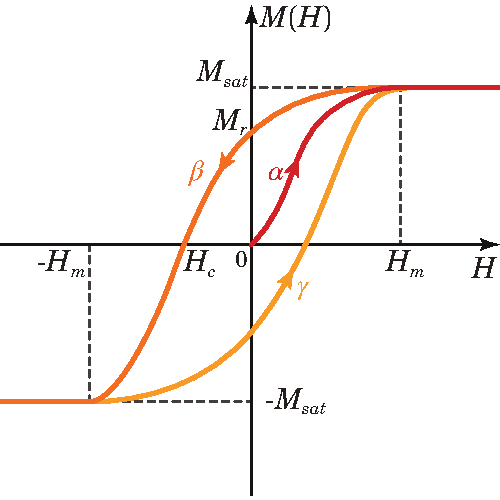
\includegraphics[width=0.75\textwidth]{images/chp12/chp12ferromagnetigraf1.pdf}
	\end{center}
\end{minipage}
\begin{minipage}{0.49\textwidth}
	\begin{center}
		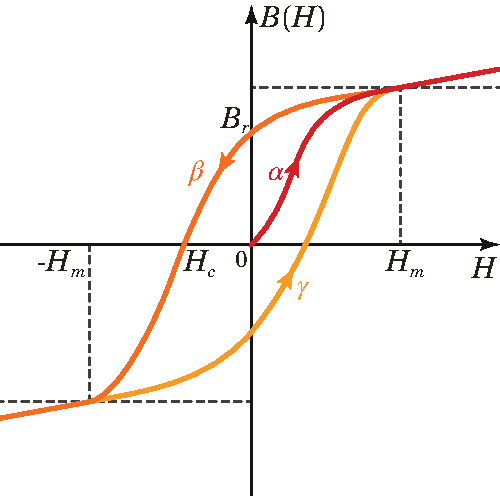
\includegraphics[width=0.75\textwidth]{images/chp12/chp12ferromagnetigraf2.pdf}
	\end{center}
\end{minipage}
Per poter \textit{smagnetizzare} completamente il materiale, ossia riportarlo ad uno stato vergine, bisogna interrompere la magnetizzazione \textit{prima} di raggiungere il livello di saturazione: in questo modo, si ottengono dei cicli sempre più stretti con i vertici sulla curva di prima magnetizzazione, fino a far convergere il ciclo allo stato vergine.
	\begin{center}
	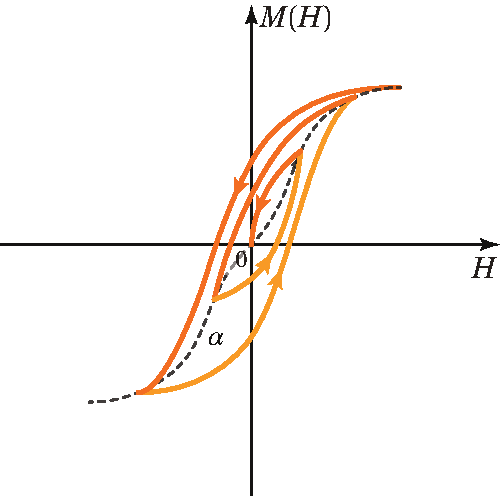
\includegraphics[width=0.5\textwidth]{images/chp12/chp12ferromagnetigraf3.pdf}
\end{center}
In questo modo in realtà è possibile raggiungere un qualunque punto compreso tra le curve $\beta$ e $\gamma$: non essendo \textit{univoco} il valore che $B(H)$ (o $M(H)$) assume, la magnetizzazione di una sostanza ferromagnetica dipende dalla \textit{storia della sostanza}, oltre che dal valore di $H$.
\begin{observe}
	Il ciclo dipende dal \textit{materiale}. Ci sono materiali detti \textit{duri} in cui il ciclo di isteresi è \textit{largo} e sono adatti a diventare materiali permanenti in quanto il valore della magnetizzazione residua $M_r$ è vicino a quella di saturazione $M_{sat}$. D'altro canto, i materiali \textit{dolci} hanno un ciclo di isteresi \textit{stretto} ed è facile smagnetizzarli - per questo sono utili per costruire degli \textit{elettromagneti}, cioè magneti il cui campo può essere facilmente controllato dalla quantità di corrente che scorre nelle bobine che lo costituiscono.
	%TODO: disegno?
\end{observe}
\paragraph{Seconda legge di Curie}
Una proprietà dei materiali ferromagnetici è l'esistenza di una \textit{temperatura critica}, detta \textbf{temperatura di Curie} $T_C$ tale per cui una materiale ferromagnetico che la supera diventa paramagnetico (e viceversa), con la suscettività alla temperatura $T$ che segue la \textbf{seconda legge di Curie}\index{legge!di Curie, seconda}:
\begin{equation}
		\tcboxmath[colback=yellowpastellow!30!white,drop fuzzy shadow, nobeforeafter, math upper, tcbox raise base, enhanced]{\chi_m=C\frac{\rho}{T-T_C}}
\end{equation}
dove $C$ è la \textbf{costante di Curie}\index{costante!di Curie} specifica del materiale e $\rho$ la densità.\\
Questa transizione di fase è spiegabile solo a livello quantistico-statistico tramite il \textit{modello di Ising}.